\documentclass[7pt]{article}
\usepackage[left=1in, right=1in, top=1in, bottom=1in]{geometry}
\usepackage[latin1]{inputenc}
\usepackage{amsmath}
\usepackage{amsfonts}
\usepackage{amssymb}
\usepackage{graphicx}
\author{Ben Larson}
\title{Homework 2 }
\date{Sept 14, 2016} 
\begin{document}
	\maketitle
	For this homework I developed line search algorithms as they apply to steepest decent and newton method. The algorithms I wrote were done in MATLAB and followed the description as seen in the book, Chp3 pg 60,61. \\
	I would first like to define a few terms so that I can talk about the experiments. \\
	Each experiment went through the same number of iterations to find the minimum using:
	$$ \alpha_k = LineSearch()$$
	$$ x_{k+1} = x_k + \alpha_k p_k $$
	$$repeat$$
	
	Where the search direction is defined as $p_k = -\beta_k^{-1}\triangledown f_k$  and $\beta_k^{-1} = I$ for steepest decent and $\beta_k^{-1}= \triangledown^2f(x_k)$ for newton methods. \\
	This homework focused on finding the optimal $\alpha_k$. This is accomplished by passing an intial guess for $\alpha_k$ through a system of wolfe conditions:
	\begin{center}
	$$ f(x_k + \alpha*p_k) \le f(x_k)+c_1*\alpha \triangledown f_k^{T} p_k $$ Sufficient decrease condition. This condition will only allow $\alpha$ values that reduce our function value after our step. 
	$$ \triangledown f(x_k+\alpha_k p_k)^{T} p_k \ge c_2 \triangledown f_k^T p_k $$ Curvature condition. This condition is to check if we can make bigger step sizes. 
	\end{center}
	
	I define $\triangledown f_k^T p_k$ as the directional derivative below. 
	\begin{center}
	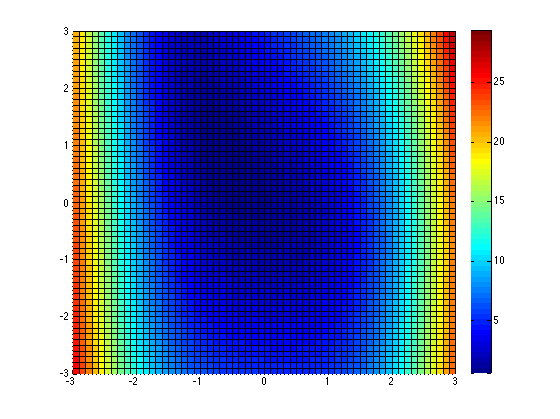
\includegraphics[width = 10cm]{fx1}\\
	Image of the value map of $f_1(x_1,x_2)$. From this we can kind of get an estimate of the minimum using this range of values(-3:3).\\
	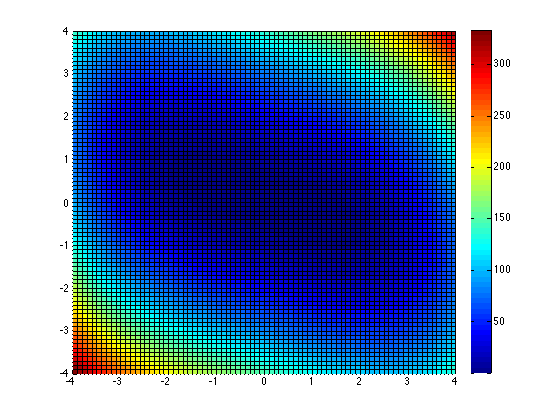
\includegraphics[width = 10cm]{fx2}\\
	Image of the value map for $f_2(x_1,x_2)$. We again can get a general idea of the minimizer for the ranges of (-4:4). 
\end{center}
	
	\section{Code} 
	This is how I selected an $\alpha$ for the optimization methods. 
	There were parts of the algorithm that was put in the book that I couldn't figure out. Mostly the zoom method produced results I didn't expect. Such as when my $\alpha$ did not satisfy the sufficient decrease condition and continued to try and find a new smaller alpha. After 40 iterations of this I just stopped it and used whatever alpha it had reached. For steepest descent I picked my first alpha to be unreasonably large (100) this is so that I will for sure break the sufficient decrease condition and force my algorithm to find smaller steps. For newton method my initial alpha was 1 as suggested in the book.\\
	
	Line Search
	\begin{enumerate}
	\item Chose an initial $\alpha_0 = 0$ and $\alpha_1$ between 0 and max. 
	loop 
		\item check if sufficient decrease, if not then use zoom 
		\item check curvature conditions, if not then use zoom
		\item check directional derivative is negative if not, use zoom
		\item if none of these conditions were met, then chose a new $\alpha_i$, larger. 
		
		\end{enumerate}
		
			Zoom
		\begin{enumerate}
		\item interpolate for a trial value $\alpha_j$between  $\alpha_i$. The input lets say is the interval: a (low alpha) and b (high alpha). 
		\item if sufficient decrease not met, decrease the highest step; b = $\alpha_j$
		\item else, check curvature conditions. and if ok this is the new $\alpha_i$  b = a 
		\item if both fail try a new alpha in the range of input $\alpha_i$ and $\alpha_{max}$
	\end{enumerate}
	
	\section{Steepest Descent}
	
	f1 using [1,0] as initial point. 
	\begin{center}
		\begin{tabular}{ | l | l | l | l | l |}
			\hline
			iteration & location & directional derivative & step length & f(x) \\ \hline
			 1& [-0.280,-0.299] & [-3.277,-0.765] & 0.3907 & 0.978\\ \hline
			 2& [-0.370,0.812] & [-0.058,0.711] & 1.5626 & 0.851\\ \hline
			 3& [-0.902,0.567]  & [-1.361,-0.627] & 0.3907 & 0.831\\ \hline
			 4& [-0.533,0.667] & [1.887,0.514] & 0.1954 & 0.616\\
			\hline
			\end{tabular}
			\end{center}
			
			
			f1 using [-1,1] as initial condition. 
				\begin{center}
					\begin{tabular}{ | l | l | l | l | l |}
						\hline
						iteration & location & directional derivative & step length & f(x) \\ \hline
						1& -1.1,-0.2 & -2.7,-0.9 & 0.78 & 2.35\\ \hline
						2& 0.3,0.15 & 3.8,1.1  & 0.39 & 1.4\\ \hline
						3& -0.7,-0.2 & -1.3,-0.5  & 0.78 & 1.23\\ \hline
						4& -0.15,0.13 & 1.5,1.04  & 0.39 & 0.87\\
						\hline
					\end{tabular}
				\end{center}
			
			f2 using [1,0] as initial point. Step length stagnant between iterations, but still decreasing. Maybe already close to the local minimum (see graphs and location above). 
			\begin{center}
				\begin{tabular}{ | l | l | l | l | l |}
					\hline
					iteration & location & directional derivative & step length & f(x) \\ \hline
					1& [0.6,-0.5]  &[-3.2,-6]  & 0.097 & 1.21\\ \hline
					2& [0.85,0.04]& [1.7,6.4] & 0.097 & 1.13\\ \hline
					3& [0.59,-0.35] & [-2.7,-5.9] & 0.09 & 1.069\\ \hline
					4& [0.76,0.06] &[1.78,6.0]  & 0.09 & 0.998\\
					\hline
				\end{tabular}
				
			\end{center}
			
			f2 using [1,-1] as center point. Does not reach a minimum if compared to min above. Maybe this is because of the slow zig zag down gradients (see directional derivatives). 
				\begin{center}
					\begin{tabular}{ | l | l | l | l | l |}
						\hline
						iteration & location & directional derivative & step length & f(x) \\ \hline
						1& 1.2,0.17  & 2.8,12  & 0.09 & 4.0\\ \hline
						2& 0.6,-0.8 & -6,-10  & 0.0978 & 3.88\\ \hline
						3& 1, 0.2 & 3.5,11.7 & 0.0978 & 3.67\\ \hline
						4& 0.5,-0.8 & -4.9,-10.9  & 0.0978 & 3.54\\
						\hline
					\end{tabular}
				\end{center}
				
				
				f3 using [1,0,0] as center point. This method seems to work well for this function. 
				\begin{center}
					\begin{tabular}{ | l | l | l | l | l |}
						\hline
						iteration & location & directional derivative & step length & f(x) \\ \hline
						1& 0.9,0.09,0 & -2,15,0  & 0.0062 & 0.46\\ \hline
						2& 0.98,0.06,-0.001 & -0.5,-3.7,-0.1 & 0.062 & 0.42\\ \hline
						3& 0.972,0.08,-0.002 & -0.9,0.8,-0.1 & 0.0123 & 0.4186\\ \hline
						4& 0.9,0.06,0-0.003 & -0.7,-1.4,-0.1 & 0.0123 & 0.4151\\
						\hline
					\end{tabular}
				\end{center}
				
				
				f3 using [1,-1,0] as center point 
					\begin{center}		
						\begin{tabular}{ | l | l | l | l | l |}
							\hline
							iteration & location & directional derivative & step length & f(x) \\ \hline
							1& 0.8,0.33,0.012 & -17,215,2  & 0.0062 & 7.4\\ \hline
							2& 0.9,0.003,0.006 & 3.2,-53,-0.9  & 0.0062 & 0.6\\ \hline
							3& 0.9,0.08,0.005 & -1.7,13,05,-0.14 & 0.0062 & 0.38\\ \hline
							4& 0.9,0.06,0.004 & -0.5,-3.2,-0.2 & 0.0062 & 0.3565\\
							\hline
						\end{tabular}
					\end{center}
					
	%%%%%%%%%%%%%%%%%%%%%%%%%%%%%%%%%%%%%%%%%%%%%%%%%%%%%
	\section{Newton Method}
	
	f1 using [1,0] as initial point. 
	\begin{center}
		\begin{tabular}{ | l | l | l | l | l |}
			\hline
			iteration & location & directional derivative & step length & f(x) \\ \hline
			1& [0.66,-0.200] & [-0.6,-0.4] & 0.5 & 1.7727\\ \hline
			2& [0.3687,-0.176] & [-0.5,0.05] & 0.5 & 1.342 \\ \hline
			3& [-0.481,0.271] & [-0.8,0.4] & 1.0 & 0.658\\ \hline
			4& [-0.733,0.757]  & [-0.25,0.5] & 1.0001 & 0.58\\
			\hline
		\end{tabular}
	\end{center}
	
	
	f1 using [1,-1] as initial point. However matlab threw error "matrix singular". I checked the eigen values of the hessian, the smallest was 0. The algorithm still made small decreases towards a minimum however. Possibly matlab fixes the singular problem on it's own(modifying the hessian). 
		\begin{center}
			\begin{tabular}{ | l | l | l | l | l |}
				\hline
				iteration & location & directional derivative & step length & f(x) \\ \hline
				1& 0.7 -1  & -.5, 0  & & 2.07\\ \hline
				2&  0.3, -1 &  & & 1.69\\ \hline
				3& 0.32, -1 &  & & 1.69\\ \hline
				4& 0.078,-1 &  & & 1.62\\
				\hline
			\end{tabular}
		\end{center}
		
		
		
		f2 using [1,0] as initial point 
		\begin{center}
			\begin{tabular}{ | l | l | l | l | l |}
				\hline
				iteration & location & directional derivative & step length & f(x) \\ \hline
				1& [0.9,-0.01]  & [-0.33,-0.22] &  0.0625 & 1.15\\ \hline
				2& [0.9,-0.02] & [-0.3,-0.2] & 0.0625 & 1.02\\ \hline
				3& [0.9,-0.03] & [-3,-0.1]  & 0.0625 & 0.912\\ \hline
				4& [0.9,-0.04] & [-0.3,-0.17] & 0.0625 & 0.8109\\
				\hline
			\end{tabular}
		\end{center}
		
		
		f2 using [1,-1] as center point. 
			\begin{center}
				\begin{tabular}{ | l | l | l | l | l |}
					\hline
					iteration & location & directional derivative & step length & f(x) \\ \hline
					1& 0.9,-0.9 & -0.2,-0.7 & 0.0625 & 3.97\\ \hline
					2& 0.95,-0.90 & -0.3,0.7  & 0.0625 & 3.34\\ \hline
					3& 0.93,-0.86 & -0.3,0.6  & 0.0625 & 2.94\\ \hline
					4& 0.9,-0.8 & -0.3,0.6  & 0.0625 & 2.6\\
					\hline
				\end{tabular}
			\end{center}
		
					f3 using [1,0,0] as center point .The problem with this function and method was that sufficient decrease was not obtained.
		\begin{center}
			\begin{tabular}{ | l | l | l | l | l |}
				\hline
				iteration & location & directional derivative & step length & f(x) \\ \hline
				1& 0.9,0,0  & -1,0,0  & 0.0078 & 0.984\\ \hline
				2& 0.9,0,0  & -0.9,0,0 & 0.0078 & 0.9691\\ \hline
				3& 0.9,0, 0 & -0.9,0,0 & 0.0078 & 0.954\\ \hline
				4& 0.9,0,0 & -0.9,0,0 & 0.0078 & 0.9392\\
				\hline
			\end{tabular}
		\end{center}
		
		f3 using [1,-1,0] as center point 
	\begin{center}
		\begin{tabular}{ | l | l | l | l | l |}
			\hline
			iteration & location & directional derivative & step length & f(x) \\ \hline
			1& 0.9,-0.9,0 & -1,1,0 & 0.0078 & 114.19\\ \hline
			2& 0.9,-0.9, 0& -0.9,0.9,0  & 0.0078  & 112.4\\ \hline
			3& 0.9,-0.9,0 & -0.9,0.9,0  & 0.0078  & 110.6\\ \hline
			4& 0.9,-0.9,0 & -0.97,0.97,0 & 0.0078 & 108.94\\
			\hline
		\end{tabular}
	\end{center}
			
		
		%%%%%%%%%%%%%%%%%%%%%%%%%%%%%%%%%%%%%%%%%%%%%%%%%%%%%
	\section{Modified Newton}
	What modified Newton means is that you correct for the possibility that the hessian matrix is not positive definite. MATLAB threw errors saying my matrix was singular. I believe this is similar to the positive definite problem. My solution was to check the eigenvalues of the hessian. If $any( eigen values <= 0)$ then I added a small $\epsilon * I$ to the hessian matrix. 
	$$ \triangledown f_k^2 = \triangledown f_k^2 + \epsilon I $$
	
	f1 using [1,0] as initial point. 
		\begin{center}
			\begin{tabular}{ | l | l | l | l | l |}
				\hline
				iteration & location & directional derivative & step length & f(x) \\ \hline
				1& [0.6,-0.2] & [-0.6,-0.4]  & 0.5 & 1.77\\ \hline
				2&  [0.3,-0.2]&[-0.6,0.04]  & 0.5 & 1.34\\ \hline
				3& [-0.4,0.27] & [-0.8,0.4]  & 1.0 & 0.65\\ \hline
				4& [-0.7,0.7] & [-0.2,0.4] & 1.0001 & 0.58\\
				\hline
			\end{tabular}
		\end{center}
		
		
		
		f1 using [1,-1] as intial point  
			\begin{center}
				\begin{tabular}{ | l | l | l | l | l |}
					\hline
					iteration & location & directional derivative & step length & f(x) \\ \hline
					1& 0.7,-1 & -0.5,9.2e-6  & 0.5 & 2.07\\ \hline
					2& 0.3,-0.9 & -0.4,0.002  & 1.0 & 1.69\\ \hline
					3& 0.05,-0.8 & 0.14 & 1.0 & 1.45\\ \hline
					4& -0.6,0.4 & -0.6,1.3  & 1.0  & 0.59\\
					\hline
				\end{tabular}
			\end{center}
			
	
	f2 using [1,0] as initial point 
		\begin{center}
			\begin{tabular}{ | l | l | l | l | l |}
				\hline
				iteration & location & directional derivative & step length & f(x) \\ \hline
				1& [0.9,-0.01] & [-0.3,-0.2]  & 0.0625 & 1.15\\ \hline
				2& [0.95,-0.02] & [-0.3,-0.2] & 0.0625 & 1.02\\ \hline
				3& [0.9,-0.03] & [-0.31,-0.18] & 0.0625 & 0.9120\\ \hline
				4& [0.9,-0.04] & [-0.3,-0.17] & 0.0625 & 0.81\\
				\hline
			\end{tabular}
		\end{center}
		
		f2 using [1,-1] as center point. 
				\begin{center}
					\begin{tabular}{ | l | l | l | l | l |}
						\hline
						iteration & location & directional derivative & step length & f(x) \\ \hline
						1& 0.9,-0.9 & -0.2,-0.7 & 0.0625 & 3.97\\ \hline
						2& 0.95,-0.90 & -0.3,0.7  & 0.0625 & 3.34\\ \hline
						3& 0.93,-0.86 & -0.3,0.6  & 0.0625 & 2.94\\ \hline
						4& 0.9,-0.8 & -0.3,0.6  & 0.0625 & 2.6\\
						\hline
					\end{tabular}
				\end{center}

		f3 using [1,0,0] as center point.The problem with this function and method was that sufficient decrease was not obtained. I see it getting stuck in my code when trying to find a new alpha that satisfies the sufficient decrease and curvature conditions. I forced my code to stop after a certain step length was found (hence no change in alpha between iterations). 
	\begin{center}
		\begin{tabular}{ | l | l | l | l | l |}
			\hline
			iteration & location & directional derivative & step length & f(x) \\ \hline
			1& 0.9,0,0  & -1,0,0  & 0.0078 & 0.984\\ \hline
			2& 0.9,0,0  & -0.9,0,0 & 0.0078 & 0.9691\\ \hline
			3& 0.9,0, 0 & -0.9,0,0 & 0.0078 & 0.954\\ \hline
			4& 0.9,0,0 & -0.9,0,0 & 0.0078 & 0.9392\\
			\hline
		\end{tabular}
	\end{center}


f3 using [1,-1,0] as center point. 	
	\begin{center}
		\begin{tabular}{ | l | l | l | l | l |}
			\hline
			iteration & location & directional derivative & step length & f(x) \\ \hline
			1& 0.9,-0.9,0 & -1,1,0 & 0.0078 & 114.19\\ \hline
			2& 0.9,-0.9, 0& -0.9,0.9,0  & 0.0078  & 112.4\\ \hline
			3& 0.9,-0.9,0 & -0.9,0.9,0  & 0.0078  & 110.6\\ \hline
			4& 0.9,-0.9,0 & -0.97,0.97,0 & 0.0078 & 108.94\\
			\hline
		\end{tabular}
	\end{center}
	
	
\end{document}